\documentclass[11pt]{article}
\usepackage[a4paper,margin=25mm,headheight=15pt,headsep=8mm,footskip=13mm]{geometry}
\usepackage[T1]{fontenc}
\usepackage[utf8]{inputenc}
\usepackage{amsmath,amsthm}
\usepackage{newtxtext,newtxmath}
\usepackage{booktabs,array,graphicx,xcolor,microtype,fancyhdr,titlesec,enumitem}
\usepackage{pdfpages,tikz}
\usetikzlibrary{arrows.meta,positioning}
\usepackage[colorlinks=true,linkcolor=black,citecolor=black,urlcolor=black]{hyperref}
\definecolor{ink}{HTML}{262522}
\definecolor{muted}{HTML}{777065}
\definecolor{gold}{HTML}{B38D4E}
\definecolor{ivory}{HTML}{FAF8F3}
\color{ink}
\hypersetup{pdftitle={Infinity One Zero Lift: The Normal Form of Projective Memory},pdfauthor={Anthony Vito Coppa},pdfsubject={Projective involution, axial lift, four-phase occurrence, and the twenty-eight-seam reader},pdfkeywords={projective memory, linear infinity, involution, K8, occurrence, exact verification}}
\pagestyle{fancy}\fancyhf{}
\fancyhead[L]{\small\scshape Infinity One Zero Lift}
\fancyhead[R]{\small\color{muted}The Normal Form of Projective Memory}
\fancyfoot[L]{\footnotesize\color{muted}A. V. Coppa / Coppalini Architecture}
\fancyfoot[R]{\footnotesize\thepage}
\renewcommand{\headrulewidth}{0.35pt}
\titleformat{\section}{\Large\bfseries}{\thesection}{.65em}{}
\titleformat{\subsection}{\large\bfseries}{\thesubsection}{.65em}{}
\titlespacing*{\section}{0pt}{13pt}{7pt}
\titlespacing*{\subsection}{0pt}{9pt}{5pt}
\setlength{\parindent}{0pt}\setlength{\parskip}{6pt}
\setlength{\abovedisplayskip}{8pt}\setlength{\belowdisplayskip}{8pt}
\setlist{nosep,leftmargin=1.4em}
\newtheorem{theorem}{Theorem}[section]
\newtheorem{proposition}[theorem]{Proposition}
\newtheorem{corollary}[theorem]{Corollary}
\theoremstyle{definition}\newtheorem{definition}[theorem]{Definition}
\newcommand{\R}{\mathbb R}\newcommand{\C}{\mathbb C}\newcommand{\Z}{\mathbb Z}\newcommand{\N}{\mathbb N}\newcommand{\PP}{\mathbb P}
\newcommand{\Id}{I}\newcommand{\ax}{\mathrm{ax}}
\newcommand{\mi}{\mathrm i}\newcommand{\tr}{\mathsf T}
\newcommand{\Dagger}{\dagger}\newcommand{\rank}{\operatorname{rank}}
\newcommand{\diag}{\operatorname{diag}}\newcommand{\Span}{\operatorname{span}}
\newcommand{\src}[1]{\par{\footnotesize\color{muted}\textit{Source:} #1}\par}
\newcommand{\lead}[1]{\textbf{#1}\par}
\newcommand{\page}{\clearpage}
\begin{document}
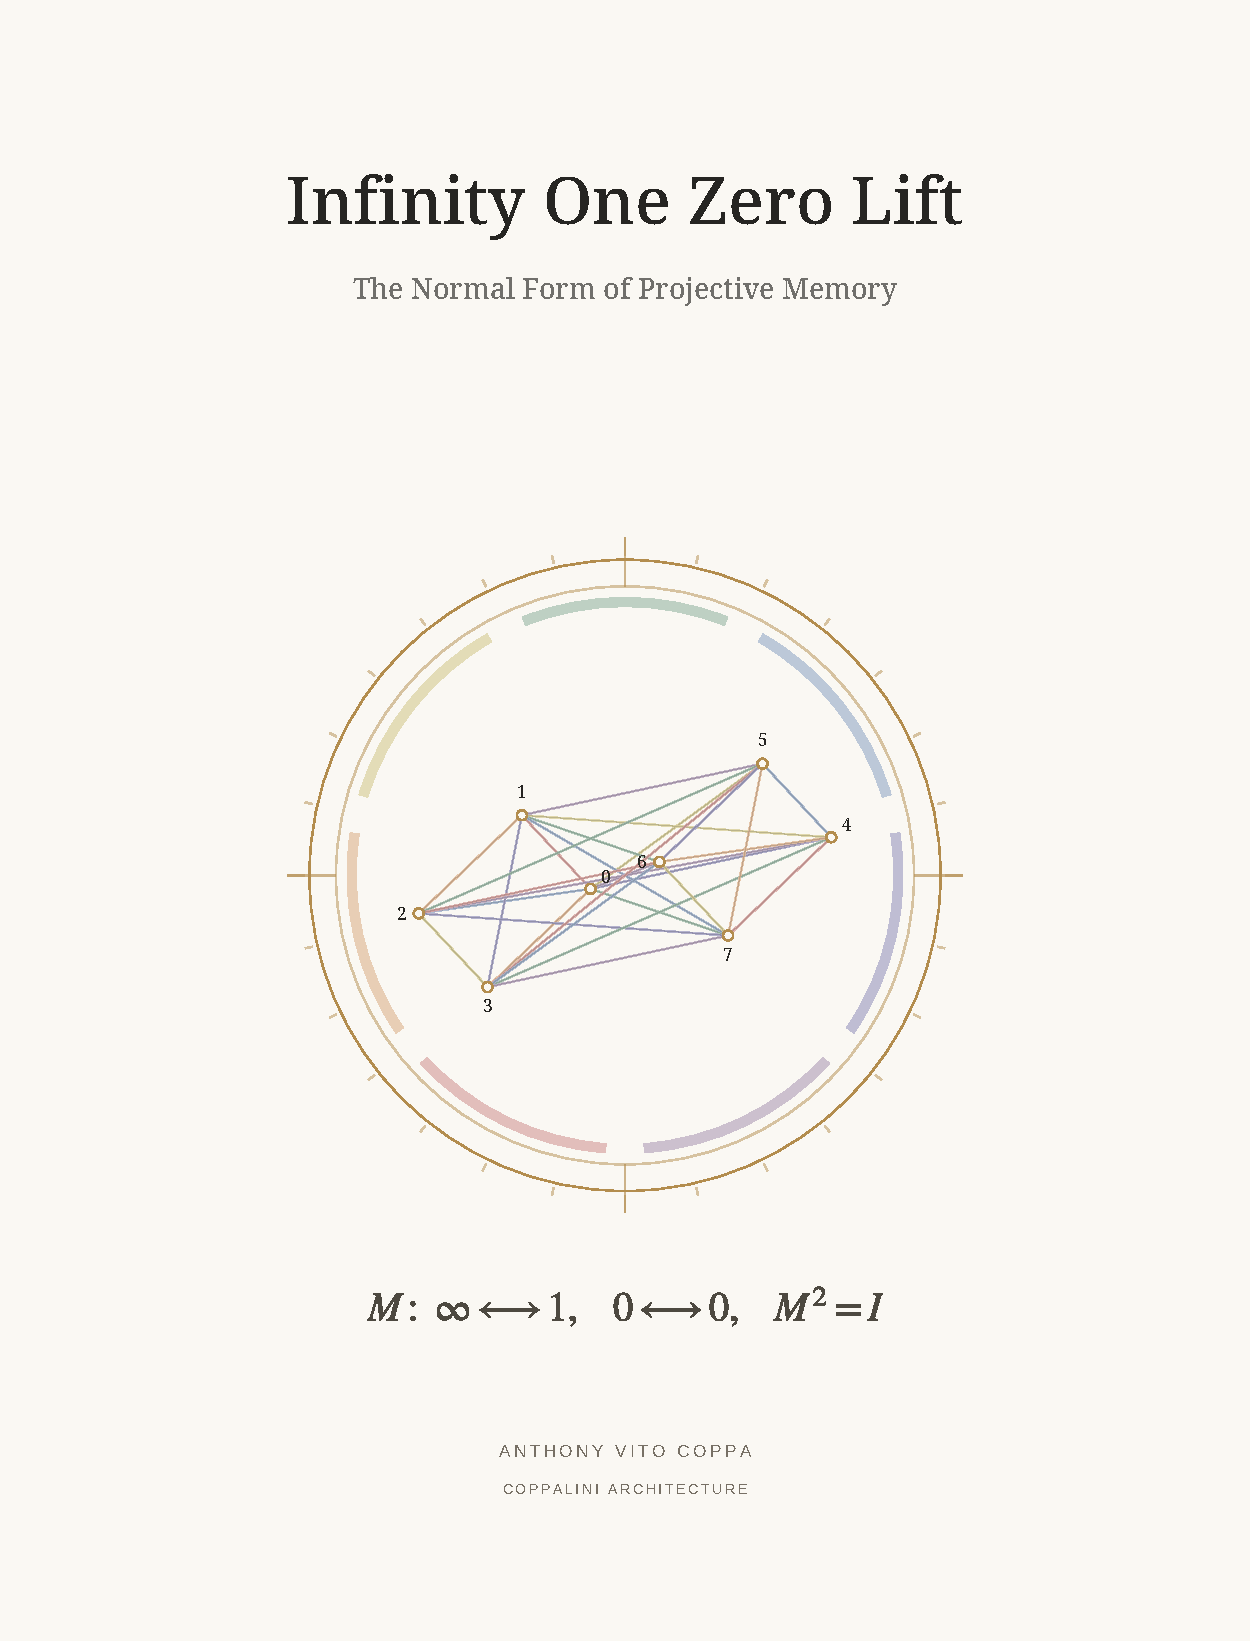
\includepdf[pages=1,fitpaper=true,pagecommand={\thispagestyle{empty}}]{assets/cover.pdf}
\setcounter{page}{1}

{\small\scshape Coppalini Architecture}\hfill{\small Working edition 0.1 / 11 November 2026}\par
\vspace{8pt}
{\LARGE\bfseries Infinity One Zero Lift}\par
{\large The Normal Form of Projective Memory}\par
Anthony Vito Coppa
\vspace{4pt}

\section*{Abstract}
A visible form can return while its occurrence advances. This paper gives an explicit normal form for that conjunction. The projective involution
\[
 M=\begin{pmatrix}1&0\\1&-1\end{pmatrix}
\]
exchanges infinity and one, fixes zero, and has a second fixed address at two. Its determinant-one complex lift has square $-I$ and fourth power $I$. Two explicit changes of coordinates connect this mirror and its four-phase lift to the existing root algebra. The axial carriage of \emph{Linear Infinity} then enters the source-defined four-state escapement. Two consecutive cycles supply eight distinct occurrence addresses; their complete comparison graph has $28=6+16+6$ edges, partitioned into seven four-edge matchings. An agreement scalar and the signed comparison record reconstruct a normalized state exactly. The resulting composition carries the displayed form, the advancing address, and the evidence needed for return in separately recoverable coordinates. The finite construction is accompanied by executable exact checks and a previously elaborated Lean subcertificate.

\section*{The result in common sense}
A clock hand can reach the same position on a later turn. Keeping the turn number makes the two visits distinguishable. Keeping the original reference and the signed differences makes the returned state reconstructible. This construction does both: it counts the traversal and preserves every pairwise comparison in the selected eight-address window.

The opening relation is
\[
\boxed{\infty\longleftrightarrow1,\qquad0\longleftrightarrow0.}
\]
The completed relation is
\[
\boxed{\text{projective return}\;\longrightarrow\;
\text{counted lift}\;\longrightarrow\;
8\text{ occurrences}\;\longrightarrow\;28\text{ comparisons}.}
\]
Every arrow below is a displayed map, a proved identity, or a declared reader. The title names this composition. The analytic and geometric steps have written proofs; the verification ledger states which parts were also executed in each checker.

\section*{Source and scope}
The construction composes \emph{Linear Infinity}~\cite{LI}, \emph{Mirror Escapement Time Lift}~\cite{METL}, Language Mechanics 011~\cite{LM11}, and the finite reconstruction of \emph{Mirror Recognition}~\cite{MR}. The initiating conversation contributes the three projective addresses and the traversal ending at its first $\mathrm{R}^{2}$ marker. Appendix A preserves that traversal. The mathematical result concerns the specified carriers, lifts, and readers; physical uses enter with their own equations and calibration.

\page
\section{Infinity, one, zero}
\lead{Infinity is a projective address. The map carries it to one exactly.}
Work on the real projective line $\PP^1(\R)$. A point is a nonzero column $(x,y)^\tr$ modulo multiplication by a nonzero real scalar. Fix
\begin{equation}
 \infty=[1:0],\qquad0=[0:1],\qquad1=[1:1].
 \label{eq:addresses}
\end{equation}
The source's ordered triples are $\mathsf L=(\infty,0,1)$ and $\mathsf T=(1,0,\infty)$. Here \emph{Light} and \emph{Time} retain their original roles as names of those triples. Their exchange is the first algebraic question.

\begin{theorem}[Unique three-address mirror]
There is exactly one projectivity satisfying $R(0)=0$, $R(\infty)=1$, and $R(1)=\infty$. It is represented by
\begin{equation}
 M=\begin{pmatrix}1&0\\1&-1\end{pmatrix},\qquad
 R([x:y])=[x:x-y],\qquad R(x)=\frac{x}{x-1}.
 \label{eq:mirror}
\end{equation}
The affine formula applies for $x\ne1$; the homogeneous formula applies everywhere. Moreover,
\begin{equation}
 M^2=I,\qquad R(\mathsf L)=\mathsf T,\qquad R(\mathsf T)=\mathsf L.
 \label{eq:triple}
\end{equation}
\end{theorem}
\begin{proof}
Let $A=\left(\begin{smallmatrix}a&b\\c&d\end{smallmatrix}\right)$ be an invertible representative. Fixing zero gives $b=0$ and $d\ne0$. Sending infinity to one gives $a=c\ne0$. Sending one to infinity gives $c+d=0$. Hence $A=aM$. Multiplication gives $M^2=I$, and componentwise application exchanges the triples.
\end{proof}

The homogeneous calculations expose the exact signs:
\begin{equation}
 M\binom10=\binom11,\qquad
 M\binom11=\binom10,\qquad
 M\binom01=\binom0{-1}.
 \label{eq:columns}
\end{equation}
Zero is fixed projectively. Its chosen vector representative changes sign.

\begin{proposition}[Two fixed addresses]
The fixed points of $R$ are precisely $0$ and $2$.
\end{proposition}
\begin{proof}
For $v=(x,y)^\tr$, the columns $v$ and $Mv$ are proportional exactly when
$\det(v,Mv)=x(x-2y)=0$. The two resulting projective points are $[0:1]$ and $[2:1]$. Infinity is exchanged with one, so supplies no additional fixed point.
\end{proof}

In the affine chart $R(x)=1+1/(x-1)$, so the limit at infinity is one. Equation~\eqref{eq:columns} realizes the same result directly, without a limiting calculation. The numerical fixed address $2$ belongs to the chosen normalization~\eqref{eq:addresses}; its coordinate is not invariant under arbitrary recharting.

\page
\section{The lift keeps the sign; the record keeps the visit}
\lead{A projective point, a lifted vector, and an occurrence have distinct return periods.}
Since $\det M=-1$, a scalar multiple $\lambda M$ has determinant one exactly when $\lambda^2=-1$. Over $\C$, the two lifts are $\pm\mi M$. Choose
\begin{equation}
 U=\mi M,\qquad U^2=-I,\qquad U^4=I.
 \label{eq:lift}
\end{equation}
Its order is exactly four. The central sign disappears in projective coordinates after two steps and survives in the vector lift.

\subsection{An explicit four-phase representation}
Let
\begin{equation}
 C_1=\begin{pmatrix}0&-1\\1&0\end{pmatrix},\qquad
 Z=\begin{pmatrix}1&\mi\\0&\mi\end{pmatrix}.
\end{equation}
Direct multiplication gives
\begin{equation}
 U=ZC_1Z^{-1},\qquad
 K=(Z^{-1})^\dagger Z^{-1}=\begin{pmatrix}1&-1\\-1&2\end{pmatrix},
 \qquad U^\dagger K U=K.
 \label{eq:unitary}
\end{equation}
The leading principal minors of $K$ are $1$ and $1$, so it is positive definite. In the $Z$ basis, the lift is the familiar unitary quarter-turn $C_1$. Its spectrum is $\{\mi,-\mi\}$. This supplies the four-step central-return algebra used by a spin-$\tfrac12$ rotation representation when its rotation action is specified. The compatible inner product is displayed rather than silently assumed to be the standard one in the original $M$ basis.

\subsection{Address return and occurrence advance}
Fix an opaque run identifier $u$ and write the $n$th occurrence as $o_n=(u,n)$. An elementary counted mirror step is
\begin{equation}
 \widehat R([v],n)=(R[v],n+1),\qquad
 \widehat R^2([v],n)=([v],n+2).
 \label{eq:countedmirror}
\end{equation}
The address returns and the visit changes. For a record updated by append,
\begin{equation}
 \mathcal H_{n+1}=\mathcal H_n\frown\langle o_n,o_{n+1}\rangle,
 \label{eq:history}
\end{equation}
the two-step record contains two additional transitions. This is the memory condition: the reference and occurrence remain available for the next comparison.

A central lift records a finite parity difference. The integer $n$ records arbitrarily many traversals. To connect the four-phase lift to an advancing geometric coordinate, we now use the published axial carriage and its escapement.
\src{The central-return/occurrence distinction is also explicit in \cite[\S VI]{METL}. The integer and Gaussian-integer identities in this section have the finite Lean witness described in Appendix B.}

\page
\section{The same mirror in the golden root}
\lead{The title mirror and the existing root mirror are connected by a stated change of coordinates.}
Retain the source matrices and their assignments:
\begin{equation}
 Q=\begin{pmatrix}1&1\\1&0\end{pmatrix},\quad
 \Omega=-C_1,\quad G=[C_1,Q]=[Q,\Omega]=\begin{pmatrix}-2&1\\1&2\end{pmatrix}.
\end{equation}
Put
\begin{equation}
 H=\frac G{\sqrt5},\qquad S=\frac{2Q-I}{\sqrt5},\qquad
 L_{\ax}=\frac{Q+2I}{\sqrt5}.
\end{equation}
The identities needed here are
\begin{align}
 Q^2&=Q+I,&G^2&=5I,&H^2=S^2&=I,& S&=HC_1,\
 L_{\ax}^2&=Q^2,&L_{\ax}^{\tr}GL_{\ax}&=G,&HL_{\ax}H&=L_{\ax}^{-1}.
 \label{eq:root}
\end{align}
For $\Phi=(1+\sqrt5)/2$, spectral decomposition of $S$ gives
$L_{\ax}=\exp((\log\Phi)S)$. Its eigenvalues are $\Phi$ and $\Phi^{-1}$.
\src{\emph{Linear Infinity}, Theorem 1 and the root construction~\cite{LI}.}

\begin{proposition}[Transported title chart]
With
\begin{equation}
 P=\begin{pmatrix}1&2+\sqrt5\\0&\sqrt5\end{pmatrix},
\end{equation}
the title mirror and its transported carriage are
\begin{equation}
 PHP^{-1}=M,\qquad
 L_M=PL_{\ax}P^{-1}=\begin{pmatrix}1+\sqrt5&-2-\sqrt5\\1&-1\end{pmatrix},
 \qquad ML_MM=L_M^{-1}.
 \label{eq:bridge}
\end{equation}
\end{proposition}
\begin{proof}
$\det P=\sqrt5\ne0$. The first two identities are direct multiplication in $\mathbb Q(\sqrt5)$. Conjugating $HL_{\ax}H=L_{\ax}^{-1}$ by $P$ proves the third.
\end{proof}

The metric travels with the coordinates:
\begin{equation}
 G_M=P^{-\tr}GP^{-1}=
 \begin{pmatrix}-2&2+\sqrt5\\2+\sqrt5&-4-2\sqrt5\end{pmatrix},
 \quad L_M^{\tr}G_ML_M=G_M.
\end{equation}
Thus equation~\eqref{eq:bridge} preserves the governing form as well as the mirror law. $P$ is the real mirror/carriage adapter; $Z$ in~\eqref{eq:unitary} is the complex phase adapter. Each transports the structure for which it was defined.

This is the first bridge of the paper: the simple $\infty\leftrightarrow1$ chart belongs to an explicitly related representation of the established mirror algebra. The second bridge is the counted passage from this four-phase representation to the axial lift.

\page
\section{Linear infinity and the four-step escapement}
\lead{One completed phase cycle releases one exact axial step.}
Let $\Psi=(1-\sqrt5)/2$ and, on the upper half-plane, define
\begin{equation}
 \xi_{\ax}(z)=\frac{\Phi-z}{z-\Psi},\qquad
 \Lambda(z)=\log\frac{\Phi}{|\xi_{\ax}(z)|},\qquad T=2\log\Phi>0.
 \label{eq:axcoord}
\end{equation}
The coordinate is finite throughout the upper half-plane. Fractional-linear substitution yields
\begin{equation}
 \xi_{\ax}(L_{\ax}z)=\Phi^{-2}\xi_{\ax}(z),\quad
 \xi_{\ax}(\mi)=-\mi\Phi,\quad
 \Lambda(L_{\ax}z)=\Lambda(z)+T,\quad\Lambda(\mi)=0.
 \label{eq:translation}
\end{equation}
The last two equalities follow by taking the logarithm of the modulus. On the quotient by $\langle L_{\ax}\rangle$, the position returns. On the cover, the real coordinate advances by $T$~\cite{LI}.

Set $P_4=\Z/4\Z$ and use the source escapement~\cite[\S V]{METL}:
\begin{equation}
 F(p,z)=\begin{cases}(p+1,z),&p=0,1,2,\\(0,L_{\ax}z),&p=3.\end{cases}
 \label{eq:escape}
\end{equation}
\begin{theorem}[Exact carry]
For $p\in\{0,1,2,3\}$ and $n\ge0$, let $c_n(p)=\lfloor(p+n)/4\rfloor$. Then
\begin{equation}
 F^n(p,z)=\bigl((p+n)\bmod4,\ L_{\ax}^{c_n(p)}z\bigr).
 \label{eq:carry}
\end{equation}
In particular, $F^4(p,z)=(p,L_{\ax}z)$.
\end{theorem}
\begin{proof}
Each successor increases the phase by one. Exactly $c_n(p)$ of the first $n$ successors cross the boundary from $3$ to $0$. Each such crossing applies $L_{\ax}$ once. This also proves the formula by induction.
\end{proof}

\subsection{Euler's phase and the recovered address}
The circle-valued read $W(z)=\exp(2\pi\mi\Lambda(z)/T)$ satisfies
$W(L_{\ax}z)=W(z)$. The independent local dial is $\mi^p$. At the fixed source $z_0=\mi$, Euclidean division gives
\begin{equation}
 n=4c+p\quad\longmapsto\quad x_n=(p,L_{\ax}^{c}\mi),\qquad
 \Lambda(L_{\ax}^{c}\mi)=cT.
 \label{eq:orbit}
\end{equation}
This map is injective: phase recovers $p$, and $\Lambda/T$ recovers $c$. On its image its exact inverse is $x_n\mapsto4\Lambda(z)/T+p$. Every four steps the local phase returns and the cycle count increases by one.

The projective pole $\infty$, the unbounded real coordinate $\Lambda$, and the integer occurrence index $n$ retain their declared types. Equations~\eqref{eq:axcoord}--\eqref{eq:orbit} supply the maps between the relevant constructions.

\page
\section{Two cycles, eight occurrences, twenty-eight seams}
\lead{Keep two turns separate, then compare every pair exactly once.}
Fix a cycle $c$. Language Mechanics 011 selects the window
\begin{equation}
 W_c=\{o_{4(c+\ell)+p}:\ell=0,1,\ p=0,1,2,3\},\qquad j=4\ell+p.
 \label{eq:window}
\end{equation}
Its eight elements are distinct. Through~\eqref{eq:orbit}, they correspond to
$(p,L_{\ax}^{c+\ell}\mi)$. The phase agrees for $j$ and $j+4$, while their axial coordinates differ by $T$~\cite{LM11,METL}.

Let $E=\R^{W_c}\cong\R^8$ be the free address carrier. A general alternating read has the unique expansion
\begin{equation}
 \omega_D=\sum_{0\le j<k\le7}D_{jk}\,e^j\wedge e^k,
 \qquad\dim\Lambda^2(E^*)=\binom82=28.
 \label{eq:28}
\end{equation}
Here $\Lambda^2$ denotes the exterior square; $\Lambda(z)$ in~\eqref{eq:axcoord} denotes a scalar coordinate. The superscript has a different, explicitly declared operation in these two expressions.

The two-cycle partition gives
\begin{equation}
 E(K_8)=E(K_4^{(c)})\sqcup E(K_{4,4})\sqcup E(K_4^{(c+1)}),
 \qquad28=6+16+6.
 \label{eq:6166}
\end{equation}

\begin{center}
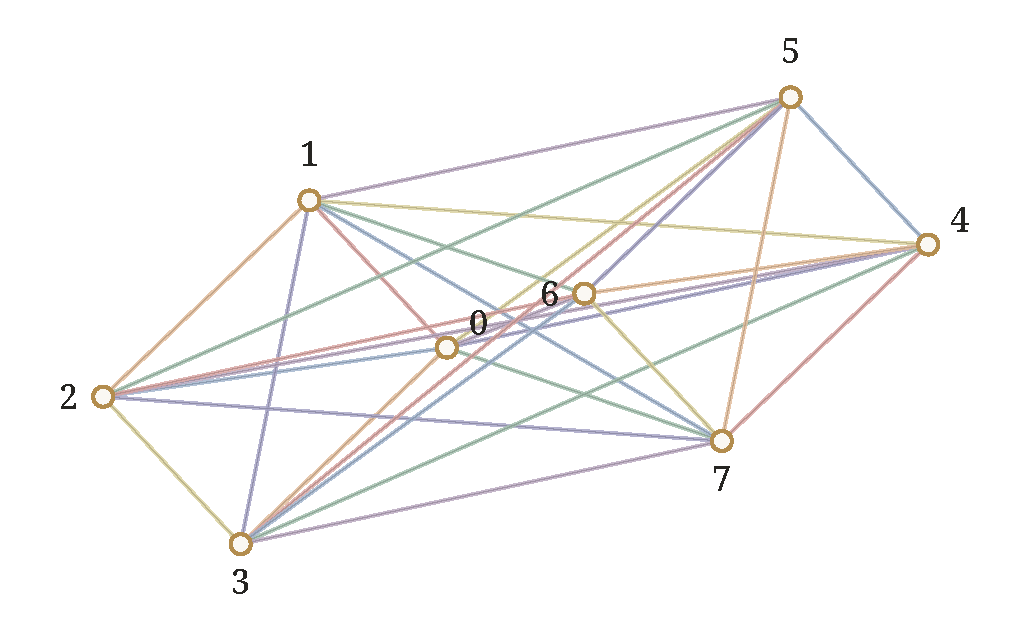
\includegraphics[width=.96\linewidth]{assets/incidence.pdf}
\end{center}
\vspace{-8pt}
{\small\textbf{Figure 1.} All eight occurrence vertices and all 28 comparisons, colored by the seven source matchings. Vertices 0--3 belong to cycle $c$; 4--7 belong to cycle $c+1$. Their positions use the recorded projection in Section~9. A crossing is not an additional vertex. Each line represents a comparison, rather than an escapement trajectory.}

The full comparison space has 28 independent coordinates. A particular reader may impose relations among their values. Section~7 states those relations explicitly for potential differences and for the reconstructing rank-two record.

\page
\section{Seven matchings and one complete scan}
\lead{Each band reads four disjoint pairs; the seven bands exhaust the window.}
Use the source relabeling $\mathcal A_8=\{\infty\}\sqcup\Z_7$. In the supplied published SVG, occurrence label $7$ is the distinguished $\infty$ slot and labels $0$--$6$ remain finite. This is a combinatorial relabeling of~\eqref{eq:window}. The projective point in~\eqref{eq:addresses} remains separately typed.

For $a\in\Z_7$, define
\begin{equation}
 \mathsf M_a=\{\{\infty,a\}\}\cup\{\{a+b,a-b\}:b=1,2,3\}.
 \label{eq:match}
\end{equation}
All finite arithmetic in this formula is modulo seven.
\begin{proposition}[Complete matching decomposition]
Each $\mathsf M_a$ has four edges and uses every vertex once. The seven matchings partition $E(K_8)$.
\end{proposition}
\begin{proof}
The finite endpoints are $a,a\pm1,a\pm2,a\pm3$, all seven residues. The edge $\{\infty,x\}$ belongs only to $\mathsf M_x$. Every finite edge $\{x,y\}$ has the unique midpoint $a=(x+y)/2$ in $\Z_7$ and one unsigned displacement $b\in\{1,2,3\}$. Thus each edge appears once.
\end{proof}
\begin{center}
\begin{tabular}{c@{\quad}cccc}
\toprule
$a$&$b=0$&$b=1$&$b=2$&$b=3$\\\midrule
0&$\infty0$&16&25&34\\
1&$\infty1$&20&36&45\\
2&$\infty2$&31&40&56\\
3&$\infty3$&42&51&60\\
4&$\infty4$&53&62&01\\
5&$\infty5$&64&03&12\\
6&$\infty6$&05&14&23\\\bottomrule
\end{tabular}
\end{center}
The notation $xy$ abbreviates an unordered edge, not multiplication.

A scanner is now defined, rather than inferred from the geometry:
\begin{equation}
 q\in\Z_{28}\longmapsto(a,b)=(q\bmod7,q\bmod4)
 \longmapsto\kappa(a,b)\in E(K_8),
\end{equation}
where $\kappa(a,0)=\{\infty,a\}$ and $\kappa(a,b)=\{a+b,a-b\}$ otherwise. The inverse coordinate is
\begin{equation}
 q=8a+21b\pmod{28}.
\end{equation}
Reduction modulo seven and four verifies both residues, proving the Chinese-remainder bijection. This gives a complete scan~\cite[\S6]{LM11}. The occurrence counter $n$ and scan counter $q$ keep independent roles until a synchronization rule is supplied.

Let $\mathcal W=\Lambda^2(E^*)$ with its orthonormal wedge basis, and let $P_a$ select the four coordinates in $\mathsf M_a$. Then
\begin{equation}
 P_aP_b=\delta_{ab}P_a,\qquad\sum_{a=0}^{6}P_a=I_{\mathcal W},\qquad\rank P_a=4.
 \label{eq:resolution}
\end{equation}
This is the seven-band identity resolution of \emph{Mirror Recognition}~\cite[\S9]{MR}.

\page
\section{The record that returns the state}
\lead{Agreement supplies the parallel part. Signed differences supply the rest.}
Fix a normalized reference $m\in\R^8$ and a normalized state $r\in\R^8$, expressed in the same ordered occurrence basis. Define
\begin{equation}
 a=m^\tr r,\qquad D=mr^\tr-rm^\tr,\qquad
 D_{jk}=m_jr_k-m_kr_j.
 \label{eq:record}
\end{equation}
These are the signed seam components of the source reconstruction~\cite[\S8]{MR}.

\begin{theorem}[Exact reconstruction]
For $\|m\|=\|r\|=1$,
\begin{equation}
 \boxed{r=am+D^\tr m,\qquad a^2+\sum_{j<k}D_{jk}^2=1.}
 \label{eq:decoder}
\end{equation}
Consequently, the read $r\mapsto(a,D)$ is injective for fixed $m$.
\end{theorem}
\begin{proof}
$D^\tr m=(rm^\tr-mr^\tr)m=r-am$. Also,
$\sum_{j<k}(m_jr_k-m_kr_j)^2=\|m\|^2\|r\|^2-(m^\tr r)^2$,
by expanding the products and grouping the diagonal and off-diagonal terms. This gives both formulas. Equal records reconstruct equal states.
\end{proof}
Writing $B_a=\sum_{\{j,k\}\in\mathsf M_a}D_{jk}^2$ gives the exact band closure
\begin{equation}
 a^2+\sum_{a'=0}^{6}B_{a'}=1.
\end{equation}
The full signed $D$ carries the decoder. The seven energies alone omit its signs. At $D=0$, the two normalized possibilities are $r=m$ and $r=-m$; the agreement $a=1$ or $-1$ distinguishes them. The projective read identifies their ray while the signed record preserves their difference.

\subsection{Twenty-eight coordinates; reader-specific freedom}
The general space in~\eqref{eq:28} has dimension 28. Record~\eqref{eq:record} is a decomposable exterior product, with matrix rank at most two. With $m$ fixed and $r$ normalized, its allowed records have the seven continuous degrees of freedom of $S^7$. The 28 slots provide a complete redundant comparison record.

A different specialized read is $d_{jk}=s_k-s_j$. It satisfies
\begin{equation}
 d_{ij}+d_{jk}+d_{ki}=0.
 \label{eq:triangles}
\end{equation}
Conversely, if~\eqref{eq:triangles} holds on every triangle, fix $s_0=0$ and set $s_j=d_{0j}$; the triangle $(0,j,k)$ yields $d_{jk}=s_k-s_j$. Thus the potential image has dimension seven. The 56 triangle equations on 28 edge coordinates have rank 21. The graph fixes available comparisons; the reader fixes their admissible values~\cite[\S5]{LM11}.

For the uniform reference $m=(1,\ldots,1)^\tr/\sqrt8$, the reconstruction specializes to
\begin{equation}
 a=\frac{1}{\sqrt8}\sum_jr_j,\qquad D_{jk}=\frac{r_k-r_j}{\sqrt8},\qquad r_j=\frac a{\sqrt8}+\frac1{\sqrt8}\sum_kD_{kj}.
\end{equation}
Here $\sqrt8$ is exactly the normalization of eight equal reference entries.

\page
\section{The normal form and its inverse}
\lead{The complete read carries both which visit occurred and what state was read.}
The preceding maps now assemble without identifying their carriers. Here \emph{normal form} means uniquely recoverable coordinates after the reference and address conventions are fixed. Fix a run $u$, the initial axial point $\mi$, the eight-address order, and a normalized reference $m$. Each window uses the declared local label $j\mapsto o_{4c+j}$; the cycle $c$ travels in the record. For $n\in\N$ and $r\in S^7$, write $n=4c+p$ and define
\begin{equation}
 \mathcal N_m(n,r)=(p,c,a,D),\qquad a=m^\tr r,\quad D=mr^\tr-rm^\tr.
 \label{eq:nf}
\end{equation}
The projective operator display can be read from $[U^p]$; the full four-phase value is $U^p$ or $\mi^p$. The axial representative of the cycle is $L_{\ax}^{c}\mi$, and $c=\Lambda(L_{\ax}^{c}\mi)/T$.

\begin{theorem}[Projective-memory normal form]
On the image of~\eqref{eq:nf},
\begin{equation}
 \boxed{\mathcal N_m^{-1}(p,c,a,D)=(4c+p,\;am+D^\tr m).}
 \label{eq:nfinverse}
\end{equation}
The source escapement returns the phase after four successors and advances the axial representative by one $L_{\ax}$ step. Two successive cycles supply eight different occurrences. Their seven matching projectors resolve the complete 28-coordinate comparison space, while the signed record reconstructs $r$ exactly.
\end{theorem}
\begin{proof}
Euclidean division uniquely recovers $(p,c)$ from $n$ and gives $4c+p=n$. Equation~\eqref{eq:decoder} recovers $r$. Equation~\eqref{eq:carry} proves the phase return and carry, and~\eqref{eq:translation} makes different cycle addresses distinct on the selected orbit. Equation~\eqref{eq:window} therefore has eight elements. Equations~\eqref{eq:match} and~\eqref{eq:resolution} exhaust all pairs. Each component of the asserted inverse has now been supplied.
\end{proof}

The inverse is stated on the image because arbitrary tuples $(p,c,a,D)$ need not satisfy normalization or decomposability. For unit $m$, an explicit image test is
\[
 r_*:=am+D^\tr m,\qquad \|r_*\|=1,\qquad
 a=m^\tr r_*,\qquad D=mr_*^\tr-r_*m^\tr,
\]
together with $p\in\{0,1,2,3\}$ and $c\in\N$. These conditions are sufficient as well as necessary. The theorem acts on supplied window records; acquisition timing is a separate condition.

\subsection{What this closes}
The coordinate adapters and construction dependencies are
\[
 M\ \overset{P}{\longleftrightarrow}\ H,\qquad
 U\ \overset{Z}{\longleftrightarrow}\ C_1,
\]
\[
 L_{\ax}\longrightarrow F\longrightarrow W_c\longrightarrow E
 \longrightarrow\mathcal W=\Lambda^2(E^*).
\]
For fixed reference $m$, the actual state-reader maps on this carrier are
\[
 r\longmapsto(a,\omega_D)\longmapsto\bigl(a,(P_b\omega_D)_{b=0}^{6}\bigr)
 \longmapsto am+D^{\tr}m=r.
\]
The projectors recover $\omega_D$ by summation; its ordered coefficients recover $D$. $P$ and $Z$ are coordinate adapters, $F$ is the published coupling, and $W_c$ is the selected occurrence window. The normal form has a written inverse and an explicit domain. That is the exact sense of closure used in this paper.

\page
\section{The geometry of the figure}
\lead{The picture is generated from the address map. Its lines keep their declared jobs.}
On the window in~\eqref{eq:window}, use the display
\begin{equation}
 v_{\ell,p}=\left(\cos\frac{\pi p}{2},\ \sin\frac{\pi p}{2},\ \ell\right).
 \label{eq:embed}
\end{equation}
The final coordinate equals the normalized axial separation
$(\Lambda(L_{\ax}^{c+\ell}\mi)-cT)/T=\ell$. For the four integer phases, all eight triples in~\eqref{eq:embed} are integers. They form two separate four-point layers.

The checked page projection is
\begin{equation}
 A_{\rm draw}=\begin{pmatrix}1&1/5&14/5\\1/7&1&3/5\end{pmatrix}.
 \label{eq:projection}
\end{equation}
It maps the vertices to the following exact rational positions:
\begin{center}
\begin{tabular}{ccl@{\qquad}ccl}
\toprule
$j$&$(\ell,p)$&$A_{\rm draw}v_{\ell,p}$&$j$&$(\ell,p)$&$A_{\rm draw}v_{\ell,p}$\\\midrule
0&$(0,0)$&$(1,1/7)$&4&$(1,0)$&$(19/5,26/35)$\\
1&$(0,1)$&$(1/5,1)$&5&$(1,1)$&$(3,8/5)$\\
2&$(0,2)$&$(-1,-1/7)$&6&$(1,2)$&$(9/5,16/35)$\\
3&$(0,3)$&$(-1/5,-1)$&7&$(1,3)$&$(13/5,-2/5)$\\\bottomrule
\end{tabular}
\end{center}
Every projected vertex is different, and the verifier checks that none lies in the interior of an unrelated edge. Each unordered pair is drawn once, using its source matching color. Intersections of lines are unmarked. Uniform page scaling and translation finish the layout.

The displayed affine span is three-dimensional, the address carrier is eight-dimensional, and the general alternating comparison space is 28-dimensional. The drawing is a two-dimensional projection of the chosen display. It supplies incidence and address readability; no physical spatial metric is assigned to the page.

\subsection{The original double diamond}
The double diamond in \emph{Linear Infinity}, printed page 3, is a pair of proof-dependency diagrams. The first constructs $L_{\ax}$ from the root relations. The second carries the positive-projective and signed-Lorentzian readings to typed Contact. Its arrows encode dependencies~\cite{LI}. Figure 1 here instead displays the eight occurrence addresses and their complete comparison set. The two diagrams have stated, complementary functions.

\subsection{The publication frame}
The cover uses the measured 800-by-1050 Coppalini SVG frame supplied with the five published references: ivory ground, centered title and diagram, seven source-ordered colors, one equation, and author/imprint footer. Its 28 lines are generated from the same edge ledger as Figure 1. The editable SVG, projection, palette, and exact source hashes accompany the manuscript.

\page
\section{Zeno, optics, and conserved transport}
\lead{The same algebra can be used at another interface once its variables are specified.}
\subsection{Finite subdivision and its limit}
For $q=2^n$, define the two homogeneous columns $X_n=(1-q,1)^\tr$ and $Y_n=(q-1,q)^\tr$. Then
\begin{equation}
 MX_n=(1-q,-q)^\tr=-Y_n,\qquad
 [MX_n]=[Y_n],\qquad s_n=\frac{q-1}{q}=1-2^{-n}.
\end{equation}
This is the exact finite-stage correspondence for Zeno's dichotomy. As $n\to\infty$, $[X_n]\to[1:0]$ and $s_n\to1$. The homogeneous equality is algebraic; convergence uses the ordinary real topology. Thus the finite completion is the image of the projective limit. A model of motion in time additionally specifies its time parameter.

\subsection{Normalized conjugate distances}
Within the ideal paraxial thin-lens model, signed object and image distances obey
\begin{equation}
 \frac1o+\frac1{d_{\rm im}}=\frac1f.
\end{equation}
With $x=o/f$ and $y=d_{\rm im}/f$, the relation becomes $xy=x+y$, hence
\begin{equation}
 y=\frac{x}{x-1}=R(x).
\end{equation}
Object and image exchange under the same involution. The finite symmetric conjugate-distance condition is $x=y=2$, giving transverse magnification $-1$. The zero address belongs to the projective extension; the physical reciprocal-distance equation requires its nonzero, model-admissible distances. Mitochondrial microlensing enters the original conversation as a biological interface, documented independently in~\cite{Ball}; it supplies no replacement for a measured wave-optical model.

\subsection{Euler, transformation groups, and Noether}
Euler exponentiation in Section~4 makes the axial coordinate circle-valued. The transformation-group description specifies which forms a motion preserves. Noether conservation enters after an action. For the source Fermi metrics~\cite{LI}, choose either $\epsilon=+1$ or $\epsilon=-1$ and the geodesic Lagrangian
\begin{equation}
 \mathcal L_\epsilon=\tfrac12\left(\dot\delta^2+\epsilon\cosh^2\delta\,\dot\Lambda^2\right).
\end{equation}
Dots denote derivatives along an affine curve parameter. Since $\partial\mathcal L_\epsilon/\partial\Lambda=0$, its Euler--Lagrange equation gives
\begin{equation}
 p_\Lambda=\epsilon\cosh^2\delta\,\dot\Lambda,\qquad
 \frac{d p_\Lambda}{dt}=0.
\end{equation}
This is the precise conserved quantity for the supplied action. The metric signature remains attached to the chosen model. The count 28 arises from the eight-address exterior square, $\sqrt5$ from $G^2=5I$, and $\pi$ from phase-angle normalization. Each constant has its own derivation.

\page
\appendix
\section{The source traversal, ending at R²}
The initiating sequence is preserved in its original order. Its roles in this edition are as follows.

\begin{center}
\small
\begin{tabular}{@{}p{.29\linewidth}p{.65\linewidth}@{}}
\toprule
Source address&Role carried here\\\midrule
Light / Time&Ordered triples $(\infty,0,1)$ and $(1,0,\infty)$; their projective exchange is proved in Section 1.\\[4pt]
Infinity to one&Exact homogeneous endpoint map $M[1:0]=[1:1]$.\\[4pt]
Memory return&Counted visit and retained reference; Sections 2, 4, and 8 give the record and inverse.\\[4pt]
Spinor&Central lift $U^2=-I$, $U^4=I$ and the explicit compatible phase representation.\\[4pt]
Zeno&Finite-stage identity and projective limit in Section 10.\\[4pt]
Beta movement&Proposed perceptual reader interface: consecutive presentations, a memory state, and a specified temporal read.\\[4pt]
G\"odel horizon&Formal proof-reader boundary, with a theory and its provability relation specified before an incompleteness claim.\\[4pt]
Mitochondrial eye&The normalized optical equation and the independently reported microlensing observation~\cite{Ball}.\\[4pt]
Shadow vision&Proposed spatial-recognition interface with named sensory input, learning rule, and calibration.\\[4pt]
\emph{Innervisions}; \emph{Songs in the Key of Life}&Artistic references introduced in the conversation as witnesses of inner perception, temporal form, and meaningful return.\\[4pt]
$\mathrm{R}^{2}$&The user's stopping marker. The subsequent private recognition-codex account lies outside this publication.\\\bottomrule
\end{tabular}
\end{center}

\subsection*{Reader equations and their evidence}
For a perceptual application, an explicit model might have sensor event $s_n$, memory state $m_n$, update $m_{n+1}=\mathcal U(m_n,s_n)$, and read $y_n=\rho(m_n,s_n)$. Those symbols specify a place for an empirical model; a measured update law and observed response must determine its content. No such calibration is supplied by the projective matrix alone.

For the G\"odel address, the precise standard hypothesis is a consistent, effectively axiomatized theory extending sufficient arithmetic. The G\"odel--Rosser conclusion concerns a sentence undecidable in that named theory~\cite{Rosser}. Addressing a sentence and proving it are separate operations. The finite identities of this paper are exhibited directly.

The artistic references preserve the historical route of the conversation. They introduce no algebraic axioms or claims about an artist's intention. This appendix records the full requested traversal while keeping the mathematical dependencies local and checkable.

\page
\section{Verification, source custody, and reproduction}
\lead{The theorem statements determine what a passing check certifies.}
This edition carries three complementary forms of evidence.

\textbf{Written proofs.} The uniqueness and fixed points of the projectivity, the analytic axial translation, the escapement iteration, the matching decomposition, the triangle criterion, and the two inverse maps are proved in the text. The source hypotheses and coordinate adapters are displayed where used.

\textbf{Finite Lean certificate.} The unchanged file \texttt{ProjectiveReturn.lean}, at source commit \texttt{43073ed248\allowbreak bad45c94dd\allowbreak12aaa0dbc0\allowbreak0a3ec64875}, has a successful GitHub execution under Lean 4.33.0~\cite{LeanRun}. It checks the integer matrix involution, chosen endpoint maps, projective zero witness, ordered-triple exchange, Gaussian-integer central-lift powers, the general integer Zeno identity, and counted return at infinity. Its \texttt{SameProjective} predicate is a sufficient nonzero-integer scaling witness for the displayed vectors; the paper's full real projective equivalence is defined in Section 1. The certificate has not formalized the real-analysis, entire $K_8$ construction, or empirical interfaces. Lean certification applies to the elaborated statements and their definitions~\cite{LeanManual}.

\textbf{Exact executable audit.} The supplied geometry verifier was rerun: all 73 checks pass. It uses integer/rational arithmetic and $\mathbb Q(\sqrt5)$ identities, checks the complete 28-edge set against the published SVG, verifies the seven matchings and scanner, and computes ranks seven and 21 for the potential and triangle maps. All 31 manuscript-supplement checks also pass. They check the transported metric, compatible complex inner product, symbolic reconstruction, all projector identities, exact normal-form examples, and the cover's vertex/edge custody. Its full output is included. Finite examples are labeled as examples; universal claims have the proofs given above.

\subsection*{Run the checks}
From the unpacked source bundle:
\begin{verbatim}
python -m pip install -r requirements.txt
python verification/geometry_audit/verify_graph.py
python verification/verify_manuscript.py
python build_cover.py
pdflatex -halt-on-error Infinity_One_Zero_Lift.tex
pdflatex -halt-on-error Infinity_One_Zero_Lift.tex
\end{verbatim}
The pinned original Lean file and a local recheck command are provided separately. The public execution receipt is retained by source commit; it is not described as a peer review or as certification of unencoded claims.

\subsection*{Authorship and edition}
Anthony Vito Coppa supplied the original observation, the source architecture, the chosen scope, title, and publication reference. Computational assistance was used for algebraic verification, source reconciliation, composition, and typesetting. This is a composed working edition, prepared for author review; no website, repository branch, or archive was modified by its creation. The source checksum manifest fixes this package's files. The manuscript introduces no empirical parameter determination or priority assertion beyond the stated composition.

\page
\begin{thebibliography}{10}\small
\bibitem{LI} Anthony Vito Coppa. \emph{Linear Infinity: Return Without Erasure in a Minimum Two-Form Architecture}. Canonical working edition 0.1, 13 August 2026. Theorem 1; ``The double diamond''; printed pp. 12--15 and 23. Author-supplied source.

\bibitem{METL} Anthony Vito Coppa. \emph{Mirror Escapement Time Lift}. Canonical working edition 0.1, 22 August 2026. Sections II--VII, especially the escapement theorem in Section V. Author-supplied source.

\bibitem{LM11} Anthony Vito Coppa. \emph{Occurrence and the Twenty-Eight-Seam Reader: Finite Addressing, Pairwise Difference, and a Complete $7\times4$ Scan}. Language Mechanics 011, standalone edition v0.2, 29 August 2026. Sections 1--8. Author-supplied source.

\bibitem{MR} Anthony Vito Coppa. \emph{Mirror Recognition: The Minimum Symmetric Field Closure}. Final form v1.0, typeset working edition, 11 September 2026. Sections 8--9, printed pp. 16--18. Author-supplied source.

\bibitem{Audit} Anthony Vito Coppa, with computational assistance. \emph{Infinity One Zero Lift: Geometry and Template Audit}. 11 November 2026. Exact coordinate/edge ledgers, 73-check verifier, and five-cover reference lock; included in this package.

\bibitem{LeanRun} \emph{ProjectiveReturn.lean}. Coppalini Architecture repository, commit \texttt{43073ed248\allowbreak bad45c94dd\allowbreak12aaa0dbc0\allowbreak0a3ec64875}. Lean 4.33.0 execution, GitHub Actions run \texttt{43033661694}, job \texttt{130566797599}; completed successfully 11 November 2026. \href{https://github.com/Coppalini-Architecture/coppalini-architecture/actions/runs/43033661694}{Public execution receipt}. Source file preserved in this package.

\bibitem{LeanManual} The Lean development team. \emph{The Lean Language Reference}, ``Validating a Lean Proof'' and ``Axioms.'' Consulted 11 November 2026. \url{https://lean-lang.org/doc/reference/latest/ValidatingProofs/}

\bibitem{Ball} John M. Ball, Shan Chen, and Wei Li. ``Mitochondria in cone photoreceptors act as microlenses to enhance photon delivery and confer directional sensitivity to light.'' \emph{Science Advances} \textbf{8}(9), eabn2070 (2022). DOI: \href{https://doi.org/10.1126/sciadv.abn2070}{10.1126/sciadv.abn2070}.

\bibitem{Rosser} J. Barkley Rosser. ``Extensions of Some Theorems of G\"odel and Church.'' \emph{The Journal of Symbolic Logic} \textbf{1}(3), 87--91 (1936). DOI: \href{https://doi.org/10.2307/2269028}{10.2307/2269028}.
\end{thebibliography}

\vfill
\begin{center}
{\color{gold}\rule{.62\linewidth}{.4pt}}\\[12pt]
\textbf{The form returns. The occurrence advances.\\The signed record remains reconstructible.}\\[12pt]
$\displaystyle\infty\longleftrightarrow1,\qquad0\longleftrightarrow0$
\end{center}
\end{document}
